% ============================================================
%  Compilers - Parser (LL(1)) & SDT report - Team 02, Group 5
%  Compile with pdfLaTeX (Overleaf default).
%  Optional figures: put screenshots in a "figures/" folder
%  (ui_syntax_error.png, ui_success.png); placeholders appear otherwise.
% ============================================================
\documentclass[11pt,a4paper]{article}

\usepackage[utf8]{inputenc}
\usepackage[T1]{fontenc}
\usepackage{lmodern}
\usepackage[english]{babel}
\usepackage[margin=2.5cm]{geometry}
\usepackage{amsmath,amssymb}
\usepackage{booktabs,longtable,array,tabularx,multirow}
\usepackage{graphicx}
\usepackage{xcolor}
\usepackage{enumitem}
\usepackage{float}
\usepackage{caption}
\usepackage{listings}
\usepackage{tikz}
\usetikzlibrary{arrows.meta,positioning,calc}
\usepackage{fancyhdr}
\usepackage[hidelinks]{hyperref}
\usepackage{placeins}

\captionsetup{font=small,labelfont=bf}
\setlength{\parskip}{4pt}
\renewcommand{\arraystretch}{1.15}

\pagestyle{fancy}
\fancyhf{}
\fancyhead[L]{\small Compilers --- Parser \& SDT}
\fancyhead[R]{\small Team 02 \textbar{} Group 5}
\fancyfoot[C]{\thepage}

\lstset{
  basicstyle=\ttfamily\footnotesize,
  frame=single,
  breaklines=true,
  columns=fullflexible,
  backgroundcolor=\color{black!3}
}

\newcommand{\eps}{\varepsilon}
\newcommand{\nt}[1]{\textit{#1}}
\newcommand{\tk}[1]{\texttt{#1}}

\begin{document}
    % ------------------------------------------------------------
%  TITLE PAGE
% ------------------------------------------------------------
\begin{titlepage}
\centering
% Uncomment if the logo files are available in the project:
% \includegraphics[height=2.4cm]{figures/unam.png}\hspace{1cm}\includegraphics[height=2.4cm]{figures/fi.png}\\[0.6cm]
%Add logos

\includegraphics[width=0.8\textwidth]{logos.png}\\[0.02cm]
\vfill

\rule{\textwidth}{1.5pt}\\[0.5cm]
{\Large\bfseries Compilers\\[0.3cm] Parser (LL(1)) and Syntax-Directed Translation (SDT)}\\[0.5cm]
\rule{\textwidth}{1.5pt}\\[3cm]

\textit{Students:}\\[0.2cm] \quad \textit{Team:} 02\\
\textbf{Cort\'es Guill\'en Pavel Francisco} -- 118001568\\
\textbf{Cojulum Ortega Mabel Ximena} -- 321101921\\
\textbf{G\'omez Meza Jorge \'Angel} -- 118003225\\
\textbf{Monroy Tapia Jesus Alejandro} -- 321045979\\
\textbf{Villa Garcia Arely Guadalupe} -- 321000697\\[2cm]

\textit{Professor:} \textbf{Ren\'e Adri\'an D\'avila P\'erez}\\
\textit{Group:} 5 
\textit{Semester:} 2027-1\\[0.4cm]

\textit{Deadline:} November 10th, 2026
\end{titlepage}

    \newpage

\tableofcontents
\newpage

% ============================================================
\section{Introduction}
% ============================================================
Compilation is organised as a pipeline of phases, each one consuming the output of the previous one. In the first deliverable of this project we built a hand-crafted lexical analyzer (Lexer) based on a 13-state deterministic finite automaton, able to recognise 40 token types and to recover from lexical errors through Panic Mode~\cite{lexer-report}. That component answers the question \emph{``do the lexemes belong to the language?''}. It cannot answer whether the sequence of tokens forms valid statements, nor whether those statements obey basic meaning rules such as ``a variable must be declared before it is used''.

This second deliverable extends the compiler of Team 02 with two new phases:
\begin{itemize}[noitemsep]
  \item a \textbf{syntax analyzer (parser)}, which validates the token stream against a context-free grammar (CFG) and builds a parse tree; and
  \item a \textbf{semantic analyzer based on Syntax-Directed Translation (SDT)}, which traverses the tree to check declarations, uses, scopes and data types, using the symbol table shared with the Lexer.
\end{itemize}

\subsection{Objectives}
\begin{enumerate}[noitemsep]
  \item Receive as input the tokens produced by the Lexer (the parser never re-tokenises the source text).
  \item Define a grammar whose productions match the token categories of the language.
  \item Choose a parsing method, build the parse tree and define the SDT rules for semantic analysis.
  \item Read the source from a string or a file and report the line of every error.
  \item Distinguish the three possible outcomes: \emph{parsing error}, \emph{parsing success with SDT error}, and \emph{successful compilation}, justifying each one theoretically.
\end{enumerate}

\subsection{Scope}
The implementation covers lexical, syntactic and semantic analysis, the symbol table update, the integration of the full flow and a web interface. It does \emph{not} generate machine code, execute the source program or optimise code.

\subsection{Implementation approach}
The assignment offers two options: applying only the theoretical concepts seen in class (which grants extra points), or using tools and libraries that hide the process (a ``black box'')~\cite{assignment}. Our team chose the first option. The parser and the SDT were written by hand in Python, without parser generators such as PLY, SLY, YACC or Bison. The parser uses an explicit stack, an input buffer and an LL(1) table, so that every step of the algorithm can be traced and related to the theory.

\subsection{Organisation of this report}
Section~\ref{sec:theory} presents the theoretical framework. Section~\ref{sec:dev} describes the design and the implementation, applying each concept to our language. Section~\ref{sec:results} presents the results, with the theoretical argument for each output. Section~\ref{sec:conclusions} closes with conclusions and future work.

% ============================================================
\section{Theoretical Framework}
\label{sec:theory}
% ============================================================

\subsection{Syntax analysis and context-free grammars}
The syntax analyzer takes the stream of tokens produced by the lexical analyzer and verifies that it can be generated by the grammar of the language; as a by-product it produces a tree that represents the syntactic structure of the program~\cite{aho}. The syntax of programming languages is specified with \emph{context-free grammars}, a class of formal grammars introduced by Chomsky~\cite{chomsky}.

A CFG is a 4-tuple $G=(N,\Sigma,P,S)$ where $N$ is the set of non-terminals, $\Sigma$ the set of terminals (here, the token categories emitted by the Lexer), $P$ a set of productions $A\to\alpha$ with $A\in N$ and $\alpha\in(N\cup\Sigma)^{*}$, and $S\in N$ the start symbol. A \emph{derivation} rewrites non-terminals step by step; in a \emph{leftmost derivation} the leftmost non-terminal is always the one rewritten. A \emph{parse tree} shows a derivation graphically: the root is $S$, each internal node is a non-terminal whose children are the symbols on the right-hand side of the applied production, and the leaves, read from left to right, form the input string.

\subsection{Top-down parsing and LL(1) grammars}
Parsing methods are classified as top-down (the tree is built from the root towards the leaves) and bottom-up (from the leaves towards the root; LR(0), SLR(1), CLR(1), LALR(1))~\cite{aho,cooper}. A \emph{predictive} top-down parser chooses the production to apply by looking only at the next input symbol (\emph{lookahead}), so it needs no backtracking. The class of grammars that can be parsed this way with $k=1$ symbol of lookahead is called LL(1): the first \textbf{L} stands for scanning the input from \emph{left} to right, the second \textbf{L} for producing a \emph{leftmost} derivation, and the \textbf{1} for one symbol of lookahead~\cite{lewis-stearns,knuth-topdown,rosenkrantz}.

A grammar is LL(1) if, for any two distinct productions $A\to\alpha\mid\beta$:
\begin{enumerate}[noitemsep]
  \item $\mathrm{FIRST}(\alpha)\cap\mathrm{FIRST}(\beta)=\emptyset$;
  \item at most one of $\alpha,\beta$ derives $\eps$; and
  \item if $\beta\Rightarrow^{*}\eps$, then $\mathrm{FIRST}(\alpha)\cap\mathrm{FOLLOW}(A)=\emptyset$.
\end{enumerate}
LL(1) grammars cannot be left-recursive, ambiguous or contain common prefixes among the alternatives of a non-terminal.

\subsection{Grammar transformations}
\paragraph{Elimination of left recursion.} A production $A\to A\alpha\mid\beta$ makes a top-down parser loop forever, because expanding $A$ calls $A$ again without consuming input. It is replaced by the equivalent pair
\[
A\to\beta A',\qquad A'\to\alpha A'\mid\eps .
\]
We use this transformation to write the arithmetic, relational and logical expression levels.

\paragraph{Left factoring.} When two alternatives share a prefix, $A\to\alpha\beta_1\mid\alpha\beta_2$, one lookahead symbol cannot decide between them. The common prefix is extracted:
\[
A\to\alpha A',\qquad A'\to\beta_1\mid\beta_2 .
\]
This is the transformation already used in the first deliverable~\cite{lexer-report} for the productions beginning with \tk{int} and \tk{printf}, and it is applied here to \nt{DeclStmt}, \nt{DeclRest} and \nt{ArgList}.

\subsection{FIRST and FOLLOW sets}
$\mathrm{FIRST}(\alpha)$ is the set of terminals that can begin a string derived from $\alpha$ (plus $\eps$ if $\alpha\Rightarrow^{*}\eps$). $\mathrm{FOLLOW}(A)$ is the set of terminals that can appear immediately to the right of $A$ in some sentential form (with \$ marking the end of input). They are computed with the following rules~\cite{aho}:
\begin{itemize}[noitemsep]
  \item If $X$ is a terminal, $\mathrm{FIRST}(X)=\{X\}$.
  \item If $X\to\eps$, add $\eps$ to $\mathrm{FIRST}(X)$.
  \item If $X\to Y_1Y_2\ldots Y_k$, add $\mathrm{FIRST}(Y_1)\setminus\{\eps\}$ to $\mathrm{FIRST}(X)$; if $Y_1\Rightarrow^{*}\eps$ continue with $Y_2$, and so on; add $\eps$ if all $Y_i$ derive $\eps$.
  \item \$ $\in\mathrm{FOLLOW}(S)$.
  \item For $A\to\alpha B\beta$, add $\mathrm{FIRST}(\beta)\setminus\{\eps\}$ to $\mathrm{FOLLOW}(B)$.
  \item For $A\to\alpha B$, or $A\to\alpha B\beta$ with $\eps\in\mathrm{FIRST}(\beta)$, add $\mathrm{FOLLOW}(A)$ to $\mathrm{FOLLOW}(B)$.
\end{itemize}

\subsection{LL(1) parsing table and the predictive algorithm}
The table $M[A,a]$ is filled as follows: for each production $A\to\alpha$, (i) put it in $M[A,a]$ for every terminal $a\in\mathrm{FIRST}(\alpha)$; (ii) if $\eps\in\mathrm{FIRST}(\alpha)$, put it in $M[A,b]$ for every $b\in\mathrm{FOLLOW}(A)$. A cell with two productions is a conflict (the grammar is not LL(1)); an empty cell denotes a syntax error.

The table-driven parser keeps a stack (initially \$ followed by the start symbol) and an input buffer ending in \$. Let $X$ be the top of the stack and $a$ the lookahead:
\begin{enumerate}[noitemsep]
  \item if $X=a=\$$: \textbf{accept};
  \item if $X$ is a terminal and $X=a$: pop $X$ and advance the input (\emph{match});
  \item if $X$ is a terminal and $X\neq a$: \textbf{error};
  \item if $X$ is a non-terminal and $M[X,a]=X\to Y_1\ldots Y_k$: pop $X$ and push $Y_k,\ldots,Y_1$ (so that $Y_1$ is on top);
  \item if $M[X,a]$ is empty: \textbf{error}.
\end{enumerate}
Time and space are linear in the size of the input.

\subsection{Syntax-Directed Translation}
A syntax-directed definition attaches \emph{semantic rules} to the productions of a CFG, computing \emph{attributes} of the grammar symbols. An attribute is \emph{synthesized} if its value at a node depends only on the attributes of its children; it is \emph{inherited} if it depends on its parent or siblings~\cite{knuth-semantics,aho}. A \emph{syntax-directed translation scheme} embeds the semantic actions in the productions and fixes the order in which they run. A common implementation, and the one used here, is a two-step procedure: (1) the parser validates the syntax and builds the parse tree; (2) the tree is traversed in postorder (bottom-up evaluation of synthesized attributes), executing the semantic actions. Separating the two steps cleanly distinguishes a syntax failure from a semantic failure.

\subsection{Symbol table and type checking}
The \emph{symbol table} stores, for every identifier, the attributes needed by later phases (type, size, scope, line of declaration and use, memory address)~\cite{aho,cooper}. The usual operations are \texttt{Insert}, \texttt{Lookup}, \texttt{Set} and \texttt{Reset}; the latter restores the table when a block ends, implementing block scope. \emph{Type checking} verifies that each operator is applied to operands of compatible types and that the type of an expression matches the type required by its context (assignment, condition, argument). Our language uses a \emph{strict} type system with no implicit conversions.

% ============================================================
\section{Development}
\label{sec:dev}
% ============================================================

\subsection{Selection of the parsing method}
We selected a \textbf{predictive top-down LL(1) parser, without backtracking, implemented with an explicit stack}. The decision rests on three criteria:
\begin{enumerate}
  \item \textbf{Traceability for the report and the oral defence.} Recursive descent hides the derivation state in Python's call stack. With an explicit stack we can print, at every iteration, the quadruple (\emph{Step, Stack, Input, Action}), which gives exactly the theoretical argument required for each output.
  \item \textbf{Advantage over bottom-up methods.} LR-family parsers need the canonical collection of items (closure and goto) and may show shift/reduce conflicts as the language grows. The LL(1) model works directly on FIRST and FOLLOW sets with linear time and space.
  \item \textbf{Separation of syntax and semantics.} The two-step SDT procedure (parse tree first, semantic traversal second) lets us separate \emph{Parsing Success!} followed by \emph{SDT error...} from a syntactic failure.
\end{enumerate}

\subsection{Architecture and integration}
The existing package \texttt{unam.fi.compilers.g5.02} was extended, preserving the Lexer and adding the new layers. The main module orchestrates the flow and a symbol table is shared by the Lexer and the SDT (Figure~\ref{fig:flow}).

\begin{figure}[H]
\centering
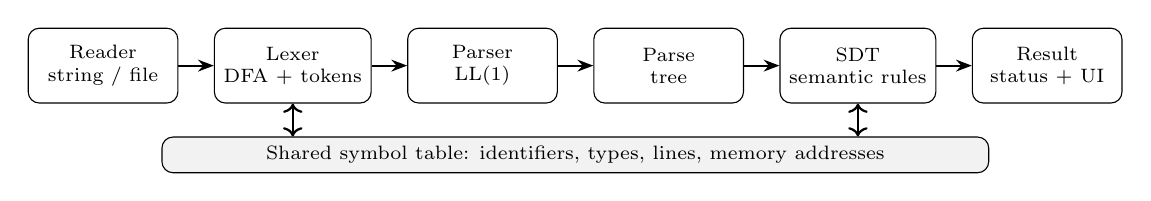
\begin{tikzpicture}[
  box/.style={draw,rounded corners,minimum width=1.9cm,minimum height=0.95cm,align=center,font=\scriptsize},
  arr/.style={-{Stealth[length=2mm]},thick},
  node distance=0.45cm]
\node[box] (r) {Reader\\string / file};
\node[box,right=of r] (l) {Lexer\\DFA + tokens};
\node[box,right=of l] (p) {Parser\\LL(1)};
\node[box,right=of p] (t) {Parse\\tree};
\node[box,right=of t] (s) {SDT\\semantic rules};
\node[box,right=of s] (o) {Result\\status + UI};
\draw[arr] (r)--(l); \draw[arr] (l)--(p); \draw[arr] (p)--(t); \draw[arr] (t)--(s); \draw[arr] (s)--(o);
\node[draw,rounded corners,fill=black!5,minimum width=10.5cm,font=\scriptsize,below=0.9cm of $(l)!0.5!(s)$] (st) {Shared symbol table: identifiers, types, lines, memory addresses};
\draw[arr,<->] (l.south) -- (l.south |- st.north);
\draw[arr,<->] (s.south) -- (s.south |- st.north);
\end{tikzpicture}
\caption{Logical flow from reading the source to presenting the results.}
\label{fig:flow}
\end{figure}

\begin{table}[H]
\centering
\small
\begin{tabularx}{\textwidth}{@{}lX@{}}
\toprule
\textbf{Module} & \textbf{Responsibility}\\
\midrule
\texttt{main.py} & Orchestrates Reader $\to$ Scanner $\to$ Parser $\to$ SDT. Keeps the lexical-only functions and adds \texttt{run\_compiler()} and \texttt{run\_compiler\_from\_file()}.\\
\texttt{io/reader.py}, \texttt{io/writer.py} & Reading of strings/files and report generation.\\
\texttt{lexer/dfa.py}, \texttt{lexer/scanner.py} & Manual lexeme recognition, positions and errors (reused from deliverable 1).\\
\texttt{parser/grammar.py} & Productions, FIRST/FOLLOW computation and predictive table.\\
\texttt{parser/ll1\_parser.py} & LL(1) stack, input buffer, terminal matching, tree construction and trace.\\
\texttt{models/ast\_node.py} & Tree node: symbol, token, children, synthesized type and line.\\
\texttt{sdt/analyzer.py} & Tree traversal and semantic checks.\\
\texttt{symbol\_table/symtab.py} & Identifiers and attributes: type, size, dimension, lines, address, declaration state.\\
\texttt{web/app.py}, templates, static & Web interface that presents the compilation results.\\
\bottomrule
\end{tabularx}
\caption{Module organisation.}
\end{table}

\paragraph{Execution flow.}
(1) The Reader obtains the source. (2) The Scanner forms the lexemes, generates tokens and records lexical errors; identifiers are inserted early in the symbol table with pending attributes. (3) The parser receives the tokens, appends the end-of-input marker \$, consults the table and builds the parse tree. (4) Only if the parser finishes successfully, the SDT traverses the tree validating declarations, uses, types and statement rules. (5) \texttt{main.py} gathers state, messages, tokens, tree, trace and symbol table, which the web application displays.

\subsection{Input: tokens from the Lexer}
The parser consumes the token list of the Lexer, whose 40 internal types are grouped for presentation into five categories (keyword, identifier, operator, constant, punctuation)~\cite{lexer-report}. For the lookahead decision the parser uses the token type or, for keywords, operators and punctuators, the specific lexeme (\tk{int}, \tk{if}, \tk{;}, \tk{==}, \dots). The terminal \textbf{id} denotes an identifier token, \textbf{const} denotes \texttt{INTEGER} or \texttt{REAL\_NUMBER}, and \textbf{lit} denotes \texttt{BOOL\_LITERAL} (\tk{True}, \tk{False}) or \texttt{STRING\_LITERAL}.

The end-of-input marker \$ is a synthetic token appended to the buffer; it is not part of the catalogue of 40 lexical tokens. The grammar was adapted to the real Lexer: identifiers are plain names such as \tk{x}, and the logical operators are the words \tk{and}, \tk{or} and \tk{not}.

\subsection{Context-free grammar}
\label{sec:grammar}
Toward a deterministic grammar, we applied left-recursion elimination (expression levels) and left factoring (declarations, calls and optional parts). Statement bodies of control structures are delimited by braces, \tk{\{ StmtList \}}, which avoids the classic dangling-else ambiguity, and every simple statement requires a terminating semicolon. The resulting grammar has 24 rules (Table~\ref{tab:grammar}); expression levels encode operator precedence, from lowest to highest: logical, relational/equality, additive, multiplicative, unary \tk{not} and primary factors.

\begin{longtable}{@{}rl@{}}
\caption{Final CFG (24 rules). Terminals in \texttt{typewriter}.}\label{tab:grammar}\\
\toprule
\textbf{\#} & \textbf{Production}\\
\midrule
\endfirsthead
\toprule \textbf{\#} & \textbf{Production}\\ \midrule
\endhead
\bottomrule
\endfoot
\multicolumn{2}{@{}l}{\textit{A. Program structure and statements}}\\
1 & $\nt{Program}\to\nt{StmtList}$\\
2 & $\nt{StmtList}\to\nt{Stmt}\ \nt{StmtList}\mid\eps$\\
3 & $\nt{Stmt}\to\nt{DeclStmt}\mid\nt{AssignStmt}\mid\nt{PrintStmt}\mid\nt{IfStmt}\mid\nt{WhileStmt}\mid\nt{ForStmt}$\\
4 & $\nt{DeclStmt}\to\nt{Type}\ \tk{id}\ \nt{DeclRest}\ \tk{;}$\\
5 & $\nt{DeclRest}\to\tk{=}\ \nt{E}\mid\eps$\\
6 & $\nt{AssignStmt}\to\tk{id}\ \tk{=}\ \nt{E}\ \tk{;}$\\
7 & $\nt{PrintStmt}\to\tk{printf}\ \tk{(}\ \nt{E}\ \nt{ArgList}\ \tk{)}\ \tk{;}$\\
8 & $\nt{ArgList}\to\tk{,}\ \nt{E}\ \nt{ArgList}\mid\eps$\\
9 & $\nt{IfStmt}\to\tk{if}\ \tk{(}\ \nt{E}\ \tk{)}\ \tk{\{}\ \nt{StmtList}\ \tk{\}}\ \nt{ElsePart}$\\
10 & $\nt{ElsePart}\to\tk{else}\ \tk{\{}\ \nt{StmtList}\ \tk{\}}\mid\eps$\\
11 & $\nt{WhileStmt}\to\tk{while}\ \tk{(}\ \nt{E}\ \tk{)}\ \tk{\{}\ \nt{StmtList}\ \tk{\}}$\\
12 & $\nt{ForStmt}\to\tk{for}\ \tk{(}\ \nt{ForInit}\ \tk{;}\ \nt{E}\ \tk{;}\ \nt{ForUpdate}\ \tk{)}\ \tk{\{}\ \nt{StmtList}\ \tk{\}}$\\
13 & $\nt{ForInit}\to\nt{Type}\ \tk{id}\ \tk{=}\ \nt{E}\mid\tk{id}\ \tk{=}\ \nt{E}$\\
14 & $\nt{ForUpdate}\to\tk{id}\ \tk{=}\ \nt{E}$\\
15 & $\nt{Type}\to\tk{int}\mid\tk{real}\mid\tk{string}\mid\tk{bool}$\\
\midrule
\multicolumn{2}{@{}l}{\textit{B. Expressions without left recursion}}\\
16 & $\nt{E}\to\nt{R}\ \nt{E}'$\\
17 & $\nt{E}'\to\nt{OpLog}\ \nt{R}\ \nt{E}'\mid\eps,\quad \nt{OpLog}\in\{\tk{and},\tk{or}\}$\\
18 & $\nt{R}\to\nt{A}\ \nt{R}'$\\
19 & $\nt{R}'\to\nt{OpRel}\ \nt{A}\ \nt{R}'\mid\eps,\quad \nt{OpRel}\in\{\tk{<},\tk{>},\tk{<=},\tk{>=},\tk{==},\tk{!=}\}$\\
20 & $\nt{A}\to\nt{T}\ \nt{A}'$\\
21 & $\nt{A}'\to\nt{OpAdit}\ \nt{T}\ \nt{A}'\mid\eps,\quad \nt{OpAdit}\in\{\tk{+},\tk{-}\}$\\
22 & $\nt{T}\to\nt{F}\ \nt{T}'$\\
23 & $\nt{T}'\to\nt{OpMult}\ \nt{F}\ \nt{T}'\mid\eps,\quad \nt{OpMult}\in\{\tk{*},\tk{/}\}$\\
24 & $\nt{F}\to\tk{(}\ \nt{E}\ \tk{)}\mid\tk{not}\ \nt{F}\mid\tk{id}\mid\tk{const}\mid\tk{lit}$\\
\end{longtable}

\subsection{FIRST and FOLLOW sets}
Applying the rules of Section~2.4 to the grammar of Table~\ref{tab:grammar} gives the sets of Table~\ref{tab:firstfollow}. Let $\mathcal{T}=\{\tk{int},\tk{real},\tk{string},\tk{bool}\}$ and $\mathrm{F}_S=\mathrm{FIRST}(\nt{Stmt})=\mathcal{T}\cup\{\tk{id},\tk{printf},\tk{if},\tk{while},\tk{for}\}$; let $\mathrm{F}_E=\{\tk{(},\tk{not},\tk{id},\tk{const},\tk{lit}\}$.

\begin{table}[H]
\centering
\small
\begin{tabularx}{\textwidth}{@{}lXX@{}}
\toprule
\textbf{Non-terminal} & \textbf{FIRST} & \textbf{FOLLOW}\\
\midrule
\nt{Program} & $\mathrm{F}_S\cup\{\eps\}$ & $\{\$\}$\\
\nt{StmtList} & $\mathrm{F}_S\cup\{\eps\}$ & $\{\tk{\}},\$\}$\\
\nt{Stmt}, \nt{DeclStmt}, \nt{AssignStmt}, \nt{PrintStmt}, \nt{IfStmt}, \nt{WhileStmt}, \nt{ForStmt} & each its own initial terminals (\nt{Stmt}: $\mathrm{F}_S$) & $\mathrm{F}_S\cup\{\tk{\}},\$\}$\\
\nt{DeclRest} & $\{\tk{=},\eps\}$ & $\{\tk{;}\}$\\
\nt{ArgList} & $\{\tk{,},\eps\}$ & $\{\tk{)}\}$\\
\nt{ElsePart} & $\{\tk{else},\eps\}$ & $\mathrm{F}_S\cup\{\tk{\}},\$\}$\\
\nt{ForInit} & $\mathcal{T}\cup\{\tk{id}\}$ & $\{\tk{;}\}$\\
\nt{ForUpdate} & $\{\tk{id}\}$ & $\{\tk{)}\}$\\
\nt{Type} & $\mathcal{T}$ & $\{\tk{id}\}$\\
\nt{E}, \nt{R}, \nt{A}, \nt{T}, \nt{F} & $\mathrm{F}_E$ & see below\\
$\nt{E}'$ & $\{\tk{and},\tk{or},\eps\}$ & $\{\tk{;},\tk{)},\tk{,}\}$\\
$\nt{R}'$ & $\{\tk{<},\tk{>},\tk{<=},\tk{>=},\tk{==},\tk{!=},\eps\}$ & $\{\tk{and},\tk{or},\tk{;},\tk{)},\tk{,}\}$\\
$\nt{A}'$ & $\{\tk{+},\tk{-},\eps\}$ & $\mathrm{FOLLOW}(\nt{R}')\cup\{\mathrm{OpRel}\}$\\
$\nt{T}'$ & $\{\tk{*},\tk{/},\eps\}$ & $\mathrm{FOLLOW}(\nt{A}')\cup\{\tk{+},\tk{-}\}$\\
\bottomrule
\end{tabularx}
\caption{FIRST and FOLLOW sets. For expressions: $\mathrm{FOLLOW}(\nt{E})=\mathrm{FOLLOW}(\nt{E}')=\{\tk{;},\tk{)},\tk{,}\}$; $\mathrm{FOLLOW}(\nt{R})$ adds $\{\tk{and},\tk{or}\}$; $\mathrm{FOLLOW}(\nt{A})$ adds the relational operators; $\mathrm{FOLLOW}(\nt{T})$ adds $\{\tk{+},\tk{-}\}$; $\mathrm{FOLLOW}(\nt{F})$ adds $\{\tk{*},\tk{/}\}$.}
\label{tab:firstfollow}
\end{table}

\subsection{LL(1) parsing table}
Following the construction rules of Section~2.5, Table~\ref{tab:ll1table} lists the production selected for each lookahead. No terminal appears in two cells of the same row: the grammar has no conflicts and is strictly LL(1). Remarkably, \tk{else} is not in $\mathrm{FOLLOW}(\nt{Stmt})$, so $\nt{ElsePart}\to\eps$ never competes with $\nt{ElsePart}\to\tk{else}\ldots$. Any combination not listed is an empty cell, i.e. a syntax error. The table is generated automatically by \texttt{parser/grammar.py}.

\begin{table}[H]
\centering
\footnotesize
\begin{tabularx}{\textwidth}{@{}lXX@{}}
\toprule
\textbf{Non-terminal} & \textbf{Production selected} & \textbf{Lookahead terminals}\\
\midrule
\nt{Program} & $\to\nt{StmtList}$ & $\mathrm{F}_S\cup\{\$\}$\\
\nt{StmtList} & $\to\nt{Stmt}\ \nt{StmtList}$ & $\mathrm{F}_S$\\
 & $\to\eps$ & $\tk{\}},\$$\\
\nt{Stmt} & $\to\nt{DeclStmt}$ / \nt{AssignStmt} / \nt{PrintStmt} / \nt{IfStmt} / \nt{WhileStmt} / \nt{ForStmt} & $\mathcal{T}$ / \tk{id} / \tk{printf} / \tk{if} / \tk{while} / \tk{for}\\
\nt{DeclRest} & $\to\tk{=}\ \nt{E}$ \quad | \quad $\to\eps$ & \tk{=} \quad | \quad \tk{;}\\
\nt{ArgList} & $\to\tk{,}\ \nt{E}\ \nt{ArgList}$ \quad | \quad $\to\eps$ & \tk{,} \quad | \quad \tk{)}\\
\nt{ElsePart} & $\to\tk{else}\ \tk{\{}\nt{StmtList}\tk{\}}$ \quad | \quad $\to\eps$ & \tk{else} \quad | \quad $\mathrm{F}_S\cup\{\tk{\}},\$\}$\\
\nt{ForInit} & $\to\nt{Type}\ \tk{id}\ \tk{=}\ \nt{E}$ \quad | \quad $\to\tk{id}\ \tk{=}\ \nt{E}$ & $\mathcal{T}$ \quad | \quad \tk{id}\\
\nt{Type} & $\to\tk{int}$ / \tk{real} / \tk{string} / \tk{bool} & the corresponding keyword\\
\nt{E}, \nt{R}, \nt{A}, \nt{T} & $\to\nt{R}\,\nt{E}'$, $\nt{A}\,\nt{R}'$, $\nt{T}\,\nt{A}'$, $\nt{F}\,\nt{T}'$ & $\mathrm{F}_E$\\
$\nt{E}'$ & $\to\nt{OpLog}\ \nt{R}\ \nt{E}'$ \quad | \quad $\to\eps$ & \tk{and}, \tk{or} \quad | \quad \tk{;}, \tk{)}, \tk{,}\\
$\nt{R}'$ & $\to\nt{OpRel}\ \nt{A}\ \nt{R}'$ \quad | \quad $\to\eps$ & relational ops. \quad | \quad \tk{and}, \tk{or}, \tk{;}, \tk{)}, \tk{,}\\
$\nt{A}'$ & $\to\nt{OpAdit}\ \nt{T}\ \nt{A}'$ \quad | \quad $\to\eps$ & \tk{+}, \tk{-} \quad | \quad FOLLOW($\nt{A}'$)\\
$\nt{T}'$ & $\to\nt{OpMult}\ \nt{F}\ \nt{T}'$ \quad | \quad $\to\eps$ & \tk{*}, \tk{/} \quad | \quad FOLLOW($\nt{T}'$)\\
\nt{F} & $\to\tk{(}\ \nt{E}\ \tk{)}$ / \tk{not}\ \nt{F} / \tk{id} / \tk{const} / \tk{lit} & \tk{(} / \tk{not} / \tk{id} / \tk{const} / \tk{lit}\\
\bottomrule
\end{tabularx}
\caption{Compact representation of the LL(1) parsing table $M[A,a]$ (\nt{IfStmt}, \nt{WhileStmt}, \nt{ForStmt}, \nt{DeclStmt}, \nt{AssignStmt} and \nt{PrintStmt} have a single production, selected on their first terminal).}
\label{tab:ll1table}
\end{table}

\subsection{Predictive parser implementation}
\texttt{parser/ll1\_parser.py} implements the algorithm of Section~2.5. Initially the stack holds the end marker \$ and the start symbol \nt{Program}, and a synthetic token with lexeme \$ is appended to the input buffer. At each iteration the top of the stack is compared with the lookahead: matching terminals consume input; for a non-terminal, the production in $M[X,a]$ is selected, its child nodes are created and pushed in reverse order so that they are processed from left to right. $\eps$-productions are applied through the FOLLOW sets.

The parser records a \textbf{trace} of four fields per step (\emph{Step, Stack, Input, Action}), including expansions, matches, $\eps$ applications and the exact point where an empty cell or a terminal mismatch is detected. This trace is the evidence of the algorithm, not only a success/error message.

\subsection{Parse tree}
Each tree node (\texttt{ASTNode}) keeps the grammar symbol, the token when the node is a terminal, the ordered list of children, the associated line, and the \texttt{data\_type} attribute synthesized later by the SDT. The tree preserves the structure of the derivation and is the only input of the semantic analyzer.

\subsection{Symbol table}
The table is shared by the Scanner and the SDT. The Lexer inserts every identifier it finds, but initially does not know whether it belongs to a valid declaration; the SDT completes the attributes when it confirms a declaration or detects a use.

\begin{table}[H]
\centering
\small
\begin{tabularx}{\textwidth}{@{}lX@{}}
\toprule
\textbf{Attribute} & \textbf{Meaning}\\
\midrule
\texttt{name} & Identifier name (key).\\
\texttt{type} & \texttt{int}, \texttt{real}, \texttt{bool} or \texttt{string}; starts as \texttt{TBD}.\\
\texttt{size} & Size in bytes; starts as \texttt{TBD}.\\
\texttt{dimension} & 0 for scalar variables.\\
\texttt{first\_appearance\_line} & First line where the Lexer found the identifier.\\
\texttt{declaration\_line} & Line of the declaration confirmed by the SDT; starts as \texttt{None}.\\
\texttt{line\_usage} & List of lines where the identifier is used.\\
\texttt{address} & Address assigned after a declaration is confirmed.\\
\bottomrule
\end{tabularx}
\caption{Symbol table entry attributes.}
\end{table}

Sizes are: \texttt{int} 4 bytes, \texttt{real} 8, \texttt{bool} 1 and \texttt{string} 16. The base address is \texttt{0x1000}; when a declaration is confirmed, the entry receives the current address and the next free address advances by the size of the type (e.g.\ \texttt{0x1000}, then \texttt{0x1004} after an \texttt{int}).

\paragraph{Design correction.} Testing revealed that the first version stored the first line where an identifier appeared in \texttt{declaration\_line}. An identifier only used in an assignment, or whose declaration had been rejected, could therefore look as if it had been declared. The two data were separated: \texttt{first\_appearance\_line} is a lexical fact, while \texttt{declaration\_line} is only set when the SDT confirms the declaration. This also keeps a single entry per identifier and prevents a duplicate declaration from overwriting the first valid one.

\subsection{Semantic analysis: SDT scheme}
\label{sec:sdt}
Semantic analysis runs only if the parser accepted the whole input. The analyzer traverses the parse tree in postorder, synthesizing the type of expressions and applying the rules of Table~\ref{tab:sdtrules}. Any violation synthesizes the attribute \texttt{error\_type} and triggers \texttt{SDT error...} with the line.

\begin{table}[H]
\centering
\footnotesize
\begin{tabularx}{\textwidth}{@{}>{\raggedright\arraybackslash}p{3.6cm}X@{}}
\toprule
\textbf{Production} & \textbf{Semantic rule}\\
\midrule
$\nt{DeclStmt}\to\nt{Type}\ \tk{id}\ \nt{DeclRest}\ \tk{;}$ & \texttt{Lookup(id)}: if already declared, error ``redeclared variable''. If there is an initialiser, its type must equal \texttt{Type}; otherwise error. Only then \texttt{Set(id, type, size, dimension=0)} and the address are confirmed.\\
$\nt{AssignStmt}\to\tk{id}\ \tk{=}\ \nt{E}\ \tk{;}$ & \texttt{Lookup(id)}: if type is \texttt{TBD} (or the variable is absent), error ``undeclared variable''; if $\texttt{id.type}\neq\texttt{E.type}$, error ``type mismatch in assignment''; else record the line of use.\\
$\nt{PrintStmt}\to\tk{printf}\ \tk{(}\ \nt{E}\ \nt{ArgList}\ \tk{)}\ \tk{;}$ & Evaluate the main expression and every extra argument; if any yields \texttt{error\_type}, error ``invalid printf argument''.\\
$\nt{IfStmt}$, $\nt{WhileStmt}$, $\nt{ForStmt}$ & The condition \nt{E} must have type \texttt{bool}; otherwise error. The bodies (and \nt{ForInit}, \nt{ForUpdate}, \nt{ElsePart}) are verified recursively.\\
$\nt{E},\nt{R},\nt{A},\nt{T}$ and primed forms & Combine the operand types following Table~\ref{tab:typematrix}; an invalid combination yields \texttt{error\_type}.\\
$\nt{F}\to\tk{(}\nt{E}\tk{)}$ & $\texttt{F.type}=\texttt{E.type}$.\\
$\nt{F}\to\tk{not}\ \nt{F}$ & Requires \texttt{bool}; result \texttt{bool}.\\
$\nt{F}\to\tk{const}\mid\tk{lit}\mid\tk{id}$ & \texttt{const}: \texttt{int} or \texttt{real} (if it contains a point); \texttt{lit}: \texttt{bool} or \texttt{string}; \texttt{id}: \texttt{Lookup(id).type} (error if \texttt{TBD}) and record the line of use.\\
Blocks \tk{\{ \dots\ \}} & Variables declared inside a block are removed (\texttt{Reset}) when the block ends; outer-scope variables remain visible.\\
\bottomrule
\end{tabularx}
\caption{SDT rules for statements and expressions.}
\label{tab:sdtrules}
\end{table}

\paragraph{Type compatibility.} The language is strictly typed over four primitive types; no automatic conversion between \texttt{int} and \texttt{real} is applied (Table~\ref{tab:typematrix}). Parenthesised expressions keep the type of the inner expression, and relational operators over numeric values produce \texttt{bool}.

\begin{table}[H]
\centering
\small
\begin{tabularx}{\textwidth}{@{}lXXXXX@{}}
\toprule
\textbf{Type} & \textbf{Arithmetic} (\tk{+ - * /}) & \textbf{Relational} (\tk{< > <= >=}) & \textbf{Equality} (\tk{== !=}) & \textbf{Logical} (\tk{and or not}) & \textbf{Assignment}\\
\midrule
\texttt{int} & int $\to$ int & int $\to$ bool & int $\to$ bool & forbidden & only \texttt{int}\\
\texttt{real} & real $\to$ real & real $\to$ bool & real $\to$ bool & forbidden & only \texttt{real}\\
\texttt{string} & only \tk{+}: string $\to$ string & forbidden & string $\to$ bool & forbidden & only \texttt{string}\\
\texttt{bool} & forbidden & forbidden & bool $\to$ bool & bool $\to$ bool & only \texttt{bool}\\
\bottomrule
\end{tabularx}
\caption{Semantic type compatibility matrix.}
\label{tab:typematrix}
\end{table}

\subsection{Control of outcomes}
The integrated flow (\texttt{run\_compiler(source)}) distinguishes four states (Table~\ref{tab:states}).

\begin{table}[H]
\centering
\small
\begin{tabularx}{\textwidth}{@{}lX@{}}
\toprule
\textbf{State} & \textbf{Behaviour}\\
\midrule
Lexical error & The Scanner records errors; the integrated flow stops before running the parser.\\
Syntax error & The parser rejects the input and reports the line (\texttt{Parsing error...}, \texttt{error in line n}). The SDT is not executed, so no semantic message is shown.\\
Semantic error & The parser accepts (\texttt{Parsing Success!}) but the SDT reports \texttt{SDT error...} and the line.\\
Successful compilation & Parser and SDT finish: \texttt{Parsing Success!} and \texttt{SDT Verified!}.\\
\bottomrule
\end{tabularx}
\caption{Outcome states of the integrated compiler.}
\label{tab:states}
\end{table}

\subsection{Web interface}
The web application (Flask) shows the editor with the source code, a summary (tokens, errors, lexical categories, supported types, overall status), the token table (type, category, lexeme, line, column), the parse tree, the LL(1) trace, the SDT result and the symbol table with first-appearance and declaration columns (a dash when no declaration was confirmed), plus the catalogue of the 40 token types. It is run as a module to keep relative imports working:
\begin{lstlisting}
cd <project>/Lexer
python -m develop.web.app      # then open http://127.0.0.1:5000
\end{lstlisting}

% ============================================================
\section{Results}
\label{sec:results}
% ============================================================

\subsection{Theoretical justification of each output}

\subsubsection{Output 1: \texttt{Parsing Success!} and \texttt{SDT Verified!}}
\textbf{Input:} \texttt{int x = 10;} \quad \textbf{Tokens:} \texttt{KW(int)}, \texttt{ID(x)}, \texttt{ASSIGN}, \texttt{INTEGER(10)}, \texttt{SEMICOLON}, \$.

Table~\ref{tab:trace} shows the condensed trace. The parser reaches the configuration (stack = \$, input = \$), which by the algorithm of Section~2.5 guarantees that the token string belongs to $L(G)$. The SDT then traverses the tree in postorder: the constant \texttt{10} synthesizes \texttt{int}, the type propagates up to \nt{E} through \nt{F}, \nt{T}, \nt{A}, \nt{R}; in \nt{DeclStmt}, \texttt{Lookup(x)} confirms the entry is still \texttt{TBD} (not redeclared) and \texttt{Type}=\texttt{int}=\texttt{E.type}, so \texttt{Set(x, int, 4, 0)} assigns address \texttt{0x1000}.

\begin{table}[H]
\centering
\scriptsize
\begin{tabularx}{\textwidth}{@{}rX>{\raggedright\arraybackslash}p{3.6cm}X@{}}
\toprule
\textbf{Step} & \textbf{Stack (base $\to$ top)} & \textbf{Input} & \textbf{Action}\\
\midrule
1 & \$ \nt{Program} & \tk{int x = 10 ; \$} & $\nt{Program}\to\nt{StmtList}$\\
2 & \$ \nt{StmtList} & \tk{int x = 10 ; \$} & $\nt{StmtList}\to\nt{Stmt}\ \nt{StmtList}$\\
3 & \$ \nt{StmtList} \nt{Stmt} & \tk{int x = 10 ; \$} & $\nt{Stmt}\to\nt{DeclStmt}$\\
4 & \$ \nt{StmtList} \nt{DeclStmt} & \tk{int x = 10 ; \$} & $\nt{DeclStmt}\to\nt{Type}\ \tk{id}\ \nt{DeclRest}\ \tk{;}$\\
5 & \$ \nt{StmtList} ; \nt{DeclRest} id \nt{Type} & \tk{int x = 10 ; \$} & $\nt{Type}\to\tk{int}$, then match \tk{int}\\
6 & \$ \nt{StmtList} ; \nt{DeclRest} id & \tk{x = 10 ; \$} & match \tk{id}\\
7 & \$ \nt{StmtList} ; \nt{DeclRest} & \tk{= 10 ; \$} & $\nt{DeclRest}\to\tk{=}\ \nt{E}$, then match \tk{=}\\
8 & \$ \nt{StmtList} ; \nt{E} & \tk{10 ; \$} & $\nt{E}\Rightarrow\nt{R}\Rightarrow\nt{A}\Rightarrow\nt{T}\Rightarrow\nt{F}$; $\nt{F}\to\tk{const}$ (via $M[\cdot,\tk{const}]$)\\
9 & \$ \nt{StmtList} ; \nt{E}$'$ \nt{R}$'$ \nt{A}$'$ \nt{T}$'$ const & \tk{10 ; \$} & match \tk{const}\\
10 & \$ \nt{StmtList} ; \nt{E}$'$ \nt{R}$'$ \nt{A}$'$ \nt{T}$'$ & \tk{; \$} & $\eps$-rules for $\nt{T}',\nt{A}',\nt{R}',\nt{E}'$ ($\tk{;}\in$ FOLLOW)\\
11 & \$ \nt{StmtList} ; & \tk{; \$} & match \tk{;}\\
12 & \$ \nt{StmtList} & \$ & $\nt{StmtList}\to\eps$\\
13 & \$ & \$ & \textbf{Parsing Success!}\\
\bottomrule
\end{tabularx}
\caption{Condensed LL(1) trace for \texttt{int x = 10;}.}
\label{tab:trace}
\end{table}

\begin{lstlisting}
Parsing Success!
SDT Verified!
\end{lstlisting}

\subsubsection{Output 2: \texttt{Parsing Success!} and \texttt{SDT error...}}
\textbf{Inputs:} \texttt{int x = "diez";} \quad \texttt{x = 5;} \quad \texttt{int x = 10; x = "hola";} \quad \texttt{if (10 + 20) \{ x = 1; \}}.

All of them satisfy 100\% of the syntactic rules of the CFG: in the first one, \texttt{"diez"} is a valid \nt{F} (\tk{lit}); in the second, an assignment with an identifier is a valid \nt{AssignStmt}; in the last one, \texttt{10 + 20} is a valid \nt{E} between parentheses followed by a braced body. Therefore the LL(1) parser empties the stack and prints \texttt{Parsing Success!}. The errors are context-dependent, so they cannot be expressed by a CFG; they are detected by the postorder traversal of the SDT: \texttt{int} $\ne$ \texttt{string} in the declaration; \texttt{x} still \texttt{TBD} in the assignment (undeclared); \texttt{int} $\ne$ \texttt{string} in the assignment; and the \texttt{IfStmt} rule requires \texttt{E.type = bool} but \texttt{10 + 20} synthesizes \texttt{int}.

\begin{lstlisting}
Parsing Success!
SDT error...
error in line 1
\end{lstlisting}

\subsubsection{Output 3: \texttt{Parsing error...}}
\textbf{Inputs:} \texttt{int x = * 10;} \quad \texttt{int x = 10} (missing semicolon).

For \texttt{int x = * 10;}, after matching \tk{=} the stack top is \nt{E} and the lookahead is \tk{*}; since $\tk{*}\notin\mathrm{FIRST}(\nt{E})$ the cell $M[\nt{E},\tk{*}]$ is empty (message \emph{no production for M[E, *]}), which is a syntax error. For \texttt{int x = 10}, the top of the stack is the terminal \tk{;} but the lookahead is \$, a terminal mismatch ($\tk{;}\neq\$$). In both cases the derivation cannot be completed, no valid tree exists and the SDT is \textbf{not} executed. The course instructions list \emph{Parsing error...} together with \emph{SDT error...} for the failing case~\cite{assignment}; our implementation prints only \texttt{Parsing error...} and the line, because semantic rules are attributes evaluated over a tree that does not exist when parsing fails (reporting a semantic error would be unjustified).

\begin{lstlisting}
Parsing error...
error in line 1
\end{lstlisting}

\subsection{Symbol table results}
\begin{table}[H]
\centering
\small
\begin{tabular}{@{}lllllll@{}}
\toprule
\textbf{Input} & \textbf{Name} & \textbf{Type} & \textbf{Size} & \textbf{First app.} & \textbf{Declaration} & \textbf{Address}\\
\midrule
\texttt{int x = 10;} & x & int & 4 & 1 & 1 & \texttt{0x1000}\\
\texttt{x = 5;} & x & TBD & TBD & 1 & --- & TBD\\
\texttt{int x = * 10;} & x & TBD & TBD & 1 & --- & TBD\\
\texttt{bool activo = True;} & activo & bool & 1 & 1 & 1 & \texttt{0x1000}\\
\texttt{real precio = 12.5;} & precio & real & 8 & 1 & 1 & \texttt{0x1000}\\
\bottomrule
\end{tabular}
\caption{Symbol table contents after compiling each input independently.}
\end{table}

\subsection{Manual test cases}
\begin{table}[H]
\centering
\small
\begin{tabularx}{\textwidth}{@{}>{\ttfamily}lXl@{}}
\toprule
\textbf{Input} & \textbf{Observed behaviour} & \textbf{Result}\\
\midrule
int x = 10; & Parser and SDT succeed; \texttt{x}: int, size 4, \texttt{0x1000}. & Correct\\
x = 5; & Parser succeeds; SDT reports undeclared variable. & Correct\\
int x = "diez"; & Parser succeeds; SDT detects int/string incompatibility. & Correct\\
int x = 10; int x = 20; & SDT detects redeclaration on line 2; keeps first entry. & Correct\\
int x = 10; x = "hola"; & SDT detects type mismatch in the assignment on line 2. & Correct\\
bool activo = True; & \texttt{bool} declaration accepted; size 1 byte. & Correct\\
real precio = 12.5; & \texttt{real} declaration accepted; size 8 bytes. & Correct\\
\bottomrule
\end{tabularx}
\caption{Exploratory manual tests in the web interface.}
\end{table}

\paragraph{Lexical and syntactic edge cases.}
\texttt{\_variable123} is recognised as \texttt{ID} but, isolated, the parser rejects it because it does not complete a statement; \texttt{10.25} is a \texttt{REAL\_NUMBER} and also an invalid isolated statement; \texttt{10.} is reported by the Lexer as a malformed number; \texttt{"Hola mundo} as an unclosed string; \texttt{@} as an illegal character with line and column; \texttt{""} is a valid empty \texttt{STRING\_LITERAL}, rejected by the parser if isolated; and \texttt{int x = * 10;} yields an empty LL(1) cell, so the SDT is not executed.

\subsection{Regression after corrections}
\begin{table}[H]
\centering
\small
\begin{tabularx}{\textwidth}{@{}>{\ttfamily}lX@{}}
\toprule
\textbf{Input} & \textbf{Verification}\\
\midrule
int x = * 10; & \texttt{Parsing error...} and the line; no \texttt{SDT error...}; \texttt{x}: first appearance 1, declaration ---.\\
x = 5; & \texttt{Parsing Success!} followed by \texttt{SDT error...} (undeclared); first appearance 1; declaration ---.\\
int x = 10; & \texttt{Parsing Success!} and \texttt{SDT Verified!}; first appearance 1; declaration 1; int; 4; \texttt{0x1000}.\\
\bottomrule
\end{tabularx}
\caption{Manual regression tests after the last commit.}
\end{table}

The last commit also removed \texttt{SDT error...} from the syntax-error output, separated \texttt{first\_appearance\_line} from \texttt{declaration\_line}, added distinct columns in the interface, created three tests for the new metadata and updated two tests whose expectations matched the previous behaviour.

\subsection{Automated testing}
The suite (unit and integration tests) is executed from the \texttt{develop/} folder with the virtual environment active:
\begin{lstlisting}
python -m unittest discover -s tests -t .. -v
\end{lstlisting}
The option \texttt{-t ..} sets the parent folder as package root, required because tests use relative imports (e.g.\ \texttt{from ..lexer}).

\begin{table}[H]
\centering
\small
\begin{tabular}{@{}lrr@{}}
\toprule
\textbf{Test group} & \textbf{Run} & \textbf{Passed}\\
\midrule
Parse tree (\texttt{test\_ast\_node.py}) & 5 & 5\\
Compiler pipeline (\texttt{test\_compiler\_pipeline.py}) & 5 & 5\\
Grammar (\texttt{test\_grammar.py}) & 4 & 4\\
LL(1) parser (\texttt{test\_ll1\_parser.py}) & 11 & 11\\
Main program / CLI (\texttt{test\_main.py}) & 8 & 8\\
SDT analyzer (\texttt{test\_sdt\_analyzer.py}) & 25 & 25\\
Declaration metadata (\texttt{test\_symbol\_declaration\_metadata.py}) & 3 & 3\\
Symbol table (\texttt{test\_symtab\_sdt.py}) & 10 & 10\\
Web pipeline (\texttt{test\_web\_pipeline.py}) & 6 & 6\\
\midrule
\textbf{Total} & \textbf{77} & \textbf{77}\\
\bottomrule
\end{tabular}
\caption{Automated test results: 77 run, 77 passed, 0 failed, 0 errors.}
\end{table}

\subsection{Interface evidence}
\begin{figure}[H]
\centering
\IfFileExists{figuresui_syntax_error.JPG}{\includegraphics[width=0.8\textwidth]{figuresui_syntax_error.JPG}}{\fbox{\parbox{0.7\textwidth}{\centering\vspace{2cm}Insert screenshot: \texttt{figures/ui\_syntax\_error.png}\vspace{2cm}}}}
\caption{Syntax error for \texttt{int x = * 10;}: the SDT is not executed.}
\end{figure}
\begin{figure}[H]
\centering
\IfFileExists{figuresui_success.JPG}{\includegraphics[width=0.8\textwidth]{figuresui_success.JPG}}{\fbox{\parbox{0.7\textwidth}{\centering\vspace{2cm}Insert screenshot: \texttt{figures/ui\_success.png}\vspace{2cm}}}}
\caption{Valid declaration \texttt{int x = 10;}: parser and SDT succeed.}
\end{figure}

\subsection{Version control and delivery status}
The work was developed on the branch \texttt{feature/parser-sdt}. Pull Request \#7 compares it against \texttt{main}; GitHub reports no conflicts. The relevant commits are \texttt{a204d30} (LL(1) parser foundation), \texttt{61ed95c} (symbol table extended for semantic analysis), \texttt{a9f3642} (SDT pipeline and web UI integration) and \texttt{93f7ae1} (parser error reporting and declaration metadata fix).

% ============================================================
\section{Conclusions}
\label{sec:conclusions}
% ============================================================
We extended the Lexer of Team 02 with a hand-written LL(1) parser and a semantic verifier based on SDT, using only the concepts seen in class. After eliminating left recursion and applying left factoring, the 24-rule grammar produced a conflict-free table, confirming that it is LL(1). The explicit stack and the trace turn every output into verifiable evidence of the algorithm.

The separation of phases was the central design decision. A string can fail while recognising tokens, while forming grammatical structures (context-free properties, detected in the table), or while obeying declaration and type rules (context-sensitive properties, detected by the SDT over the tree). This explains why a syntax error prevents semantic analysis, while a syntactically valid input can still be rejected by the SDT. Likewise, separating \texttt{first\_appearance\_line} from \texttt{declaration\_line} was necessary to represent correctly the difference between a lexical finding and a semantic fact.

The validation, with 77 automated tests passed and manual regression cases, shows that the three required outcomes behave as justified in Section~\ref{sec:results}.

\paragraph{Limitations and future work.} The compiler performs lexical, syntactic and semantic analysis only. Natural continuations are the generation of intermediate code (three-address code) from the validated tree, support for implicit conversions or arrays (dimension attribute), more informative syntax error messages with expected-token sets, and a recovery strategy for the parser (e.g.\ synchronising on FOLLOW sets) so that several syntax errors can be reported in one run.

% ============================================================
\begin{thebibliography}{99}
\bibitem{aho} A. V. Aho, M. S. Lam, R. Sethi, and J. D. Ullman, \emph{Compilers: Principles, Techniques, and Tools}, 2nd ed. Boston, MA, USA: Pearson/Addison-Wesley, 2006.
\bibitem{cooper} K. D. Cooper and L. Torczon, \emph{Engineering a Compiler}, 3rd ed. Cambridge, MA, USA: Morgan Kaufmann, 2022.
\bibitem{chomsky} N. Chomsky, ``On certain formal properties of grammars,'' \emph{Information and Control}, vol. 2, no. 2, pp. 137--167, 1959.
\bibitem{lewis-stearns} P. M. Lewis II and R. E. Stearns, ``Syntax-directed transduction,'' \emph{J. ACM}, vol. 15, no. 3, pp. 465--488, 1968.
\bibitem{rosenkrantz} D. J. Rosenkrantz and R. E. Stearns, ``Properties of deterministic top-down grammars,'' \emph{Information and Control}, vol. 17, no. 3, pp. 226--256, 1970.
\bibitem{knuth-topdown} D. E. Knuth, ``Top-down syntax analysis,'' \emph{Acta Informatica}, vol. 1, no. 2, pp. 79--110, 1971.
\bibitem{knuth-semantics} D. E. Knuth, ``Semantics of context-free languages,'' \emph{Math. Systems Theory}, vol. 2, no. 2, pp. 127--145, 1968.
\bibitem{lexer-report} P. F. Cort\'es Guill\'en \emph{et al.}, ``Compilers: Lexer,'' Facultad de Ingenier\'ia, UNAM, Mexico City, Mexico, Group 5, Team 02, Project Rep. 1, Oct. 2026.
\bibitem{assignment} Facultad de Ingenier\'ia, UNAM, ``Parser \& SDT: Syntax \& Semantic Analyzer,'' Compilers course, Group 5, assignment instructions, Nov. 2026.
\end{thebibliography}

\end{document}